\begin{ledgroupsized}[r]{120mm}%
\footnotesize%
\pstart%
\noindent\textbf{\"{U}berlieferung:}%
\pend%
\end{ledgroupsized}%
\begin{ledgroupsized}[r]{114mm}%
\footnotesize%
\pstart%
\parindent -6mm%
\makebox[6mm][l]{\textit{L}}%
Auszüge mit Bemerkungen aus einem verschollenen Ms. von René Descartes:\protect\index{Namensregister}{\textso{Descartes} (Cartesius, des Cartes), Ren\'{e} 1596-1650}
LH~IV 1, 4b Bl. 13-14.
1~Bog. 2\textsuperscript{o}.
Etwa 2\,\nicefrac{1}{2} S.
Textfolge: Bl. 13~r\textsuperscript{o}, 14~r \textsuperscript{o}.
Bl. 13~v\textsuperscript{o} und 14~v\textsuperscript{o} enthalten lediglich Texteinschübe zur jeweiligen Vorderseite.
% Je ein verschiedenes Wasserzeichen auf beiden Blättern.
% Aufgrund ihres komplexen Charakters werden die Diagramme sowohl als schematische Zeichnungen wie auch als Reproduktionen wiedergegeben.
\newline%
Cc 2, Nr. 1324%
\pend%
\end{ledgroupsized}%
% \vspace*{0.5em}
%
\begin{ledgroupsized}[r]{114mm}%
\footnotesize%
\pstart%
\parindent -6mm%
\makebox[6mm][l]{\textit{E\textsuperscript{1}}}%
(tlw.) \cite{01121}\textsc{R.~Descartes}, \textit{{\OE}uvres in\'{e}dites}, hrsg. von \textsc{L.\,A.~Foucher de Careil}, Bd. I, Paris 1859, S. 72-99 (mit franz\"{o}sischer \"{U}bersetzung).%
\pend%
\end{ledgroupsized}%
% \vspace*{0.5em}
%
\begin{ledgroupsized}[r]{114mm}%
\footnotesize%
\pstart%
\parindent -6mm%
\makebox[6mm][l]{\textit{E\textsuperscript{2}}}%
\cite{00120}\textsc{R.~Descartes}, \textit{{\OE}uvres}, hrsg. von \textsc{C.~Adam} und \textsc{P.~Tannery}, Bd. XI, Paris 1909, S.~621-634.%
\pend%
\end{ledgroupsized}%
%
%\normalsize
\vspace*{5mm}%
\begin{ledgroup}%
\footnotesize%
\count\Bfootins=1200
\count\Cfootins=1200
\count\Afootins=1200
\pstart%
\noindent%
\footnotesize{%
\textbf{Datierungsgr\"{u}nde:}
Zu dem sich damals im Besitz Claude Clerseliers befindlichen, heute verschollenen Nachlass Descartes' hat Leibniz wahrscheinlich erst im Februar 1676
-- spätestens aber am 24. (siehe N.~76) % LH003,04,03a_001 = Remedia et vires medicamentoruman
 -- Zugang gehabt.
Mit Descartes' Handschriften kann er sich dann bis gegen Ende seines Pariser Aufenthaltes (4. Oktober 1676) befasst haben.
(Siehe hierzu die Datierungsgründe in \cite{01122}\textit{LSB} VI,~3 N.~34, S.~386%; zudem \cite{?????}\textit{LSB} III,~1 N.~79, S.~373
.) In diesem Zeitraum müssen folglich auch die vorliegenden Auszüge entstanden sein.%
}%
\pend%
\end{ledgroup}%
%
\vspace*{8mm}% PR: Rein provisorisch !!!
% PR: Bitte als Überschrift getsalten !!!
\pstart
\noindent
[13~r\textsuperscript{o}]
\pend
\pstart%
\normalsize%
\noindent%
\centering%
% \edtext{}{\lemma{}\Afootnote{\textit{Am oberen Rand von Bl. 13~r\textsuperscript{o}:} 
Ex Manuscripto Cartesii\protect\index{Namensregister}{\textso{Descartes}, Ren\'{e} (1596-1650)} in 4\textsuperscript{o}
% }}%
\pend%
% PR: Dies ist weiterhin Teil der Überschrift !!!
\pstart%
\noindent
\centering
Problemata:
\pend%
\vspace*{0.5em}% PR: Rein provisorisch !!!
% PR: Hier beginnt der Text !!!
\pstart%
\noindent%
[\textit{Folgender kleingedruckter Text im Ms. gestrichen:}]
\pend%
\vspace*{0.5em}% PR: Rein provisorisch !!!
\footnotesize%
\pstart%
\noindent%
\edtext{}{\lemma{}\Afootnote{\textit{Am Rand:} (+ haec deleta in Mso +)\vspace{-8mm}}}%
Quare sal vi caloris cum aqua non extrahitur numquid ratio est, quia cum sit diaphanus a radiis non movetur sudor enim corporum est salsus, non enim excutitur a solo calore et est potius sedimentum ejus ex quo subtilior vapor in substantiam corporis conversus est, et videmus scilicet aquam quae diu bulliit magis salsam, quia scilicet ex ea plus vaporis dulcis exhalavit in fumum.
\pend%
\count\Bfootins=1200
\count\Cfootins=1200
\count\Afootins=1200
\pstart%
Falsum videtur quod jamjam dixi de sale. Aqua enim est aeque pellucida atque sal. Sed loco diaphani dicendum est esse
\edtext{pervium motui caloris}{\lemma{pervium motui}\Bfootnote{\textit{(1)}\ sal \textit{(2)}\ caloris \textit{L}}}
propter suam siccitatem[,] aqua vero licet motui luminis sit pervia non est tamen motui caloris (qui est in partibus paulo solidioribus aut majoribus) propter suam humiditatem; hinc forte reddi potest ratio cur aqua maris noctu luceat.
\pend%
\pstart%
Nulli quod sciam fructus salsi proveniunt, quae satis indicant sal esse valde fixum nec a sole in plantas elevari, sed nec ullae carnes salsae sunt, ne quidem piscium marinorum, quod indicat sal esse valde siccum, neque vero nisi glutinosa in carnes possunt transire.
\pend
\newpage
\pstart%
Amari sunt plerique fructus ii praecipue qui in calidiusculis regionibus nascuntur; ut nucum putamina
\edtext{malorum}{\lemma{}\Afootnote{\textit{Am Rand, gestrichen:} eodem modo aurium purgamenta fiunt.}}
aureorum etc. Abstergunt autem amara omnia vehementissime et exiccant; imo etiam exulcerant, et venarum extremitates resecant, ideo concludo esse partes in fumum quidem ab initio a calore excitatas, ideoque opacas, et nigras, (ut in nucis cortice) postea vero in arbore a partibus fluidis celeriter motis paulatim secretas et simul constipatas (unde olivae quo maturiores eo magis amarae) ac proinde quae faciunt corpus humidum crassissimum, quod se toto, respectu carnis nostrae est siccum, ideoque abstergit; illi enim quod crassissimum est in humoribus adhaeret, et sic omnia secum vehit, fluidissimis exceptis, quae relicta calefaciunt et siccant.
\pend%
\vspace{0.5em}% PR: Rein provisorisch !!!
\normalsize%
\pstart%
\edtext{}{\lemma{}\Afootnote{\textit{Am Rand:} (+ In margine ascriptum erat +) Rursus hodie talem grandinem vidi flabatque auster simul cum Borea et cum partibus turbinatis quae erant majusculae, cadebant aliae rotundae minores et aliae pulveris instar minutae informes, nisi viderentur esse ex filis simul convolutis.\vspace{-6mm}}}%
\textso{Grando. }%
Vidi hodie mense decembri grandinem in modum turbinis acuminatam, ita ut octava pars globi esse videretur, pluvia heri praecesserat, sol jam hodie apparuerat, boreas flabat, aer erat tepidus ventus gelidus. Non multum decidit. Ex quibus conjicere licet, nivis filamenta simul cum vento a Borea in guttas aquae reliquae ex pluvia hesterna et a sole in guttas coactae, incidisse, istasque guttas circumquaque congelasse, sed ita tamen ut partes calidiores ad earum centra confluerent, cumque istae guttae simul dum congelabantur, dejiciebantur versus terram agitatione dividebantur, non poterant autem ullo modo facilius dividi quam in duas partes, media autem illarum pars adhuc facilius in duas dividebatur et quarta adhuc in duas; octava autem cum proxime accederet ad globum non poterat ulterius dividi. Confirmatur guttis ita congelatis partes aquae tepidiores ad centrum confluxisse (quo posito reliqua aperta sunt). Ex eo quod alias, si bene memini viderim talem grandinem plane rotundam, sed cujus centrum magis albicans erat, extremitates
\edtext{vero}{\lemma{vero}\Bfootnote{\textit{erg. L}}}
magis pellucidae, id est magis densae, quod tunc contigisse puto, quod guttae aquae minores erant, et ventus frigidior. Nec ideo frangebantur.
\pend%
\pstart%
Grando autem quae aestate decidit, plane pellucida fit, quod ventus est subtilior.
Fit autem saepe concreta (\phantom)\hspace{-1.2mm}+~an
\edtext{cornuta \phantom(\hspace{-1.2mm}+) non}{\lemma{}\Bfootnote{cornuta\ \textbar\ , an \textit{streicht Hrsg.}\ \textbar\ confusa \textit{gestr.}\ \textbar\  \phantom(\hspace{-1.2mm}+) non \textit{L}}}
aliam ob causam,
\edtext{ni fallor}{\lemma{ni fallor}\Bfootnote{\textit{erg. L}}}
quam quod ventus illam dejiciendo congelat, et valde subito unde fit ut partes quae 1\textsuperscript{mae} illi occurruntur, citius durentur, nec ulla servetur aequalitas.
\pend%
\newpage
\pstart%
Notandum etiam est istius grandinis turbinatae grana non ita inter se fuisse aequalia, ut sunt nivis stellae, cujus ratio clara est, quod stellae nivis fiunt in continuo ideoque omnes aequales esse debent, grana vero hujus grandinis octo tantum fiunt ex una gutta quae debent inter se aequalia esse, sed ex alia majore gutta fient octo majora.
\pend%
\pstart%
Quare cum aqua fluminis crescit vel alta manet non ita ingreditur vicinas cellas ac dum descendit, nec ita dum celeriter crescit ac minuitur, quam cum lente; nempe propter eandem rationem propter quam si vas vacuum angusti orificii in aquam demergas, non ita implebitur aqua si celeriter demergas, quam si lente nec quicquam aquae ipsum ingredietur quamdiu totus erit demersus cum autem rursus ex aqua extrahes, si nondum ea sit plenum, nova aqua illud ingredietur, quippe pori et concavitates in terra vasi isti similes sunt.
\pend%
\pstart%
Quare nervus digito pulsatus duplex apparet? Nempe quod dum circulariter movetur diutius manet cum eodem respectu ad oculum cum est sursum vel deorsum, quam cum ascendit vel descendit ut planetae cum sunt stationarii. (+ ingeniose +)
\pend%
\pstart%
Quare halitus ore clauso emissus est frigidus?
Quod tunc omnes partes corporis quas tangit
\edtext{versus eandem partem}{\lemma{versus}\Bfootnote{\textit{(1)}\ easdem partes \textit{(2)}\ eandem partem \textit{L}}}
detinet immotas contra autem, cum minus fortis est illas movet adeoque est calidus, ut videmus aliquando cum magnus ventus est, et in eandem partem aequaliter \edtext{[flat],}{\lemma{flant}\Bfootnote{\textit{L \"{a}ndert Hrsg.}}}
non moveri sylvarum arbores nec vela navium sed tunc moveri cum ejus impetus remittitur vel primum incipit, et magis cum tantum levis aura flat, et hoc de halitu demonstratur ex eo, quod si ore clauso flemus versus
\edtext{propriam manum idem halitus qui in reliqua manu frigidus sentietur: in interstitiis digitorum, non admodum exacte junctorum, ita ut illa subingrediatur, calidus sentietur quia non tam validus ibi erit, et hinc patet cur pannus rimis januarum et fenestrarum appositus optime frigus impediat, etiamsi ventum non plane excludat.}%
{\lemma{propriam [...] excludat}\Cfootnote{Textüberhang auf Bl.~13~v\textsuperscript{o}.}}
\pend%
\pstart%
\textso{Arbores }infra terram inventae in Hollandia omnes ita inversae sunt, ut rami septentrionem respiciant. Si arbores proceras habere vis, ne reseca surculos plures enim renascerentur, sed eversos trunco alliga, ita enim emorientur.
\pend%
\pstart%
Dum plantantur novae arbores, rami et radices abscindi debent, radices autem ita ut fibrae quam maxime terrae insistant ita enim firmius inhaerentes novas radices agunt. 
\pend%
\newpage
\pstart%
5\textsuperscript{a} feb. 1635.\edtext{}{\lemma{}\Afootnote{\textit{Am Rand:} 1635.}}
Caecia flante cum praecedenti die etiam ninxisset, et id quod vocamus verglas cecidisset, erant autem granula hujus magnitudinis humorem cristallinum figura referentia et pellucida et uni et alteri, ex quibus notavi 6 radios brevissimos et ex albo pallidos etiam crassitiem granuli superantes. 5\textsuperscript{a} inquam feb. notavi valde varias nivis stellulas: 1\textsuperscript{o} quaedam solida hexagona talia valde pellucida polita et tenuia inaequalium magnitudinum, deinde rotulas tales: 
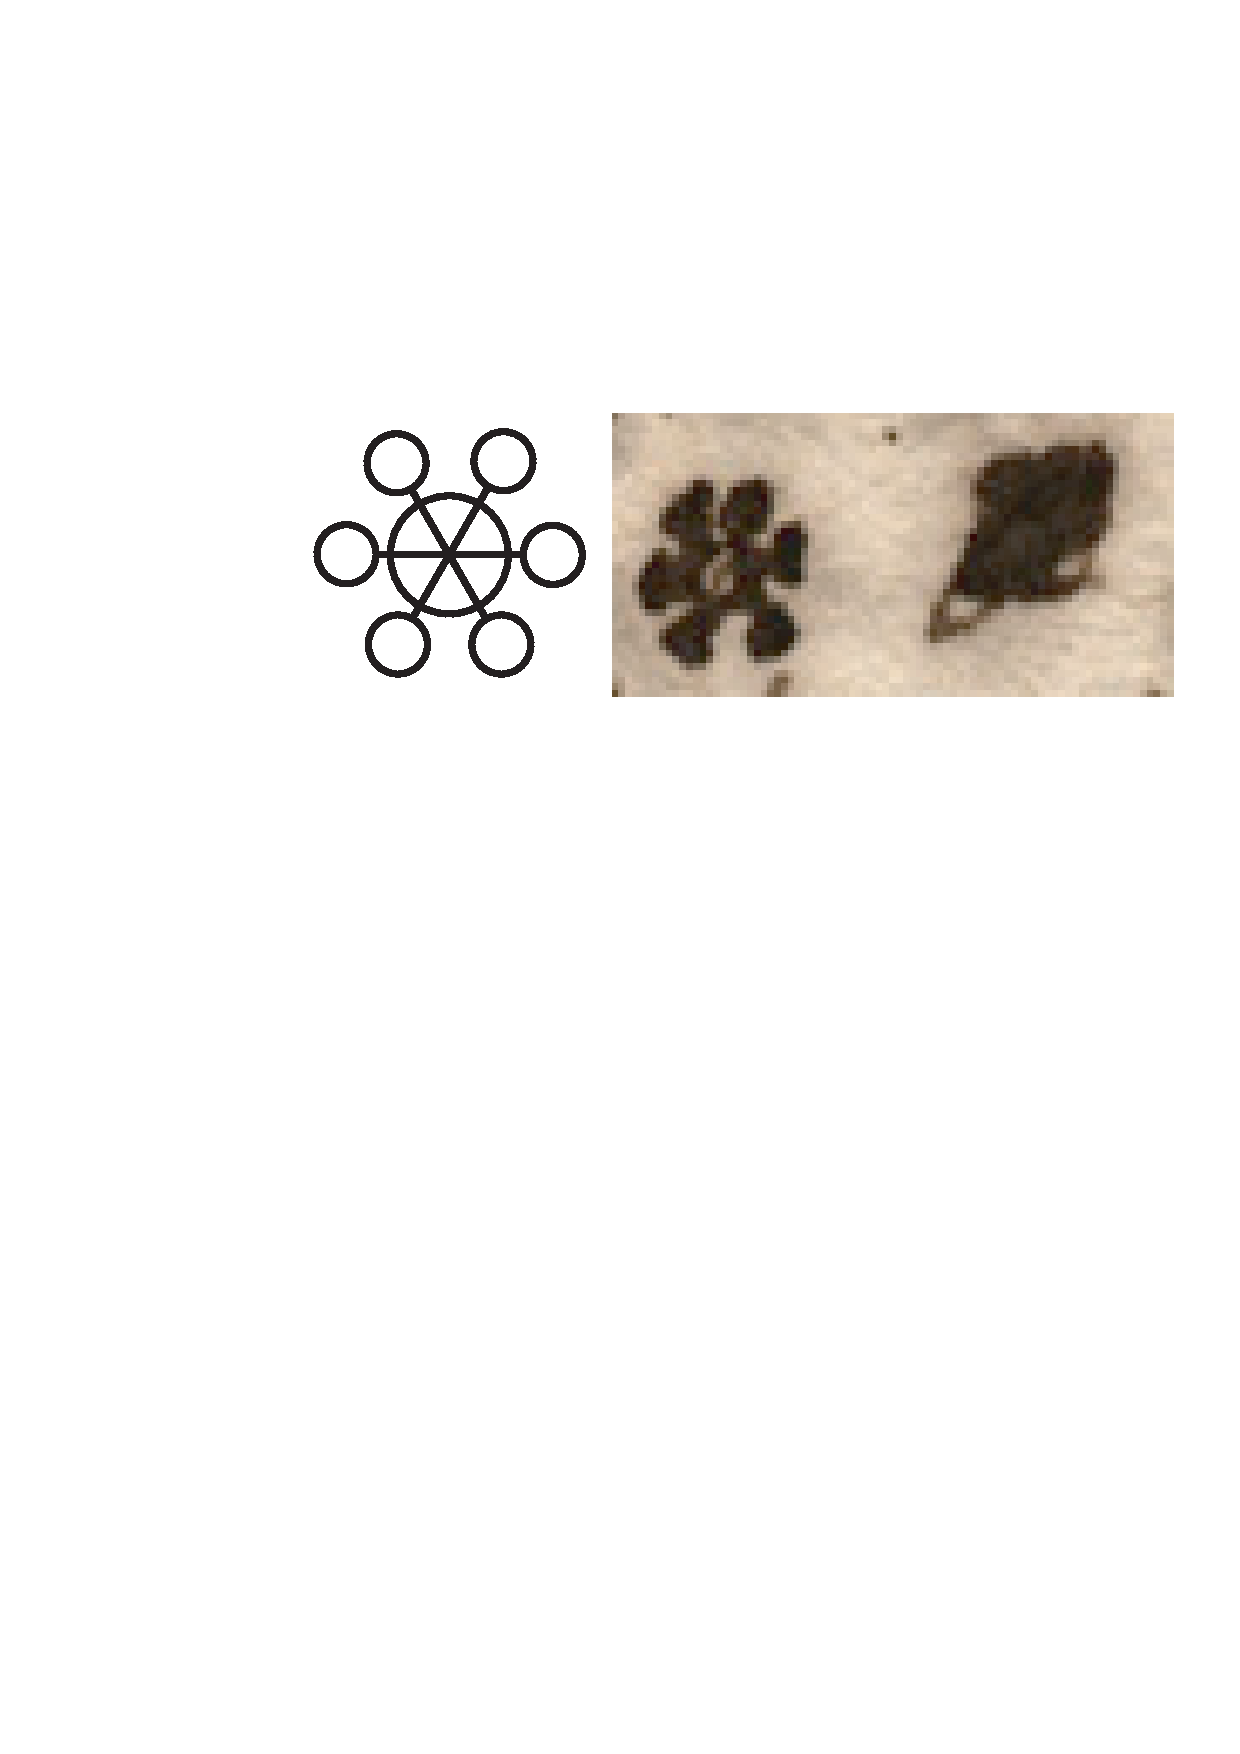
\includegraphics[width=0.1\textwidth]{images/lh0040104b_013r1.pdf}
pulchriores quam arte fingi possint, etiam cum puncto albido minutissimo in centro et fere totas pellucidas; deinde etiam alias sine puncto in centro et paulo majores cum radiis instar liliorum; ac deinde columnulas crassitiem minutae
\edtext{assiculae}{\lemma{}\Afootnote{\textit{\"{U}ber} assiculae: (+ aciculae +)}}
aequantes pellucidas, et ad utramque extremitatem habentes stellulam hoc modo: 
\rule[0mm]{0mm}{6mm}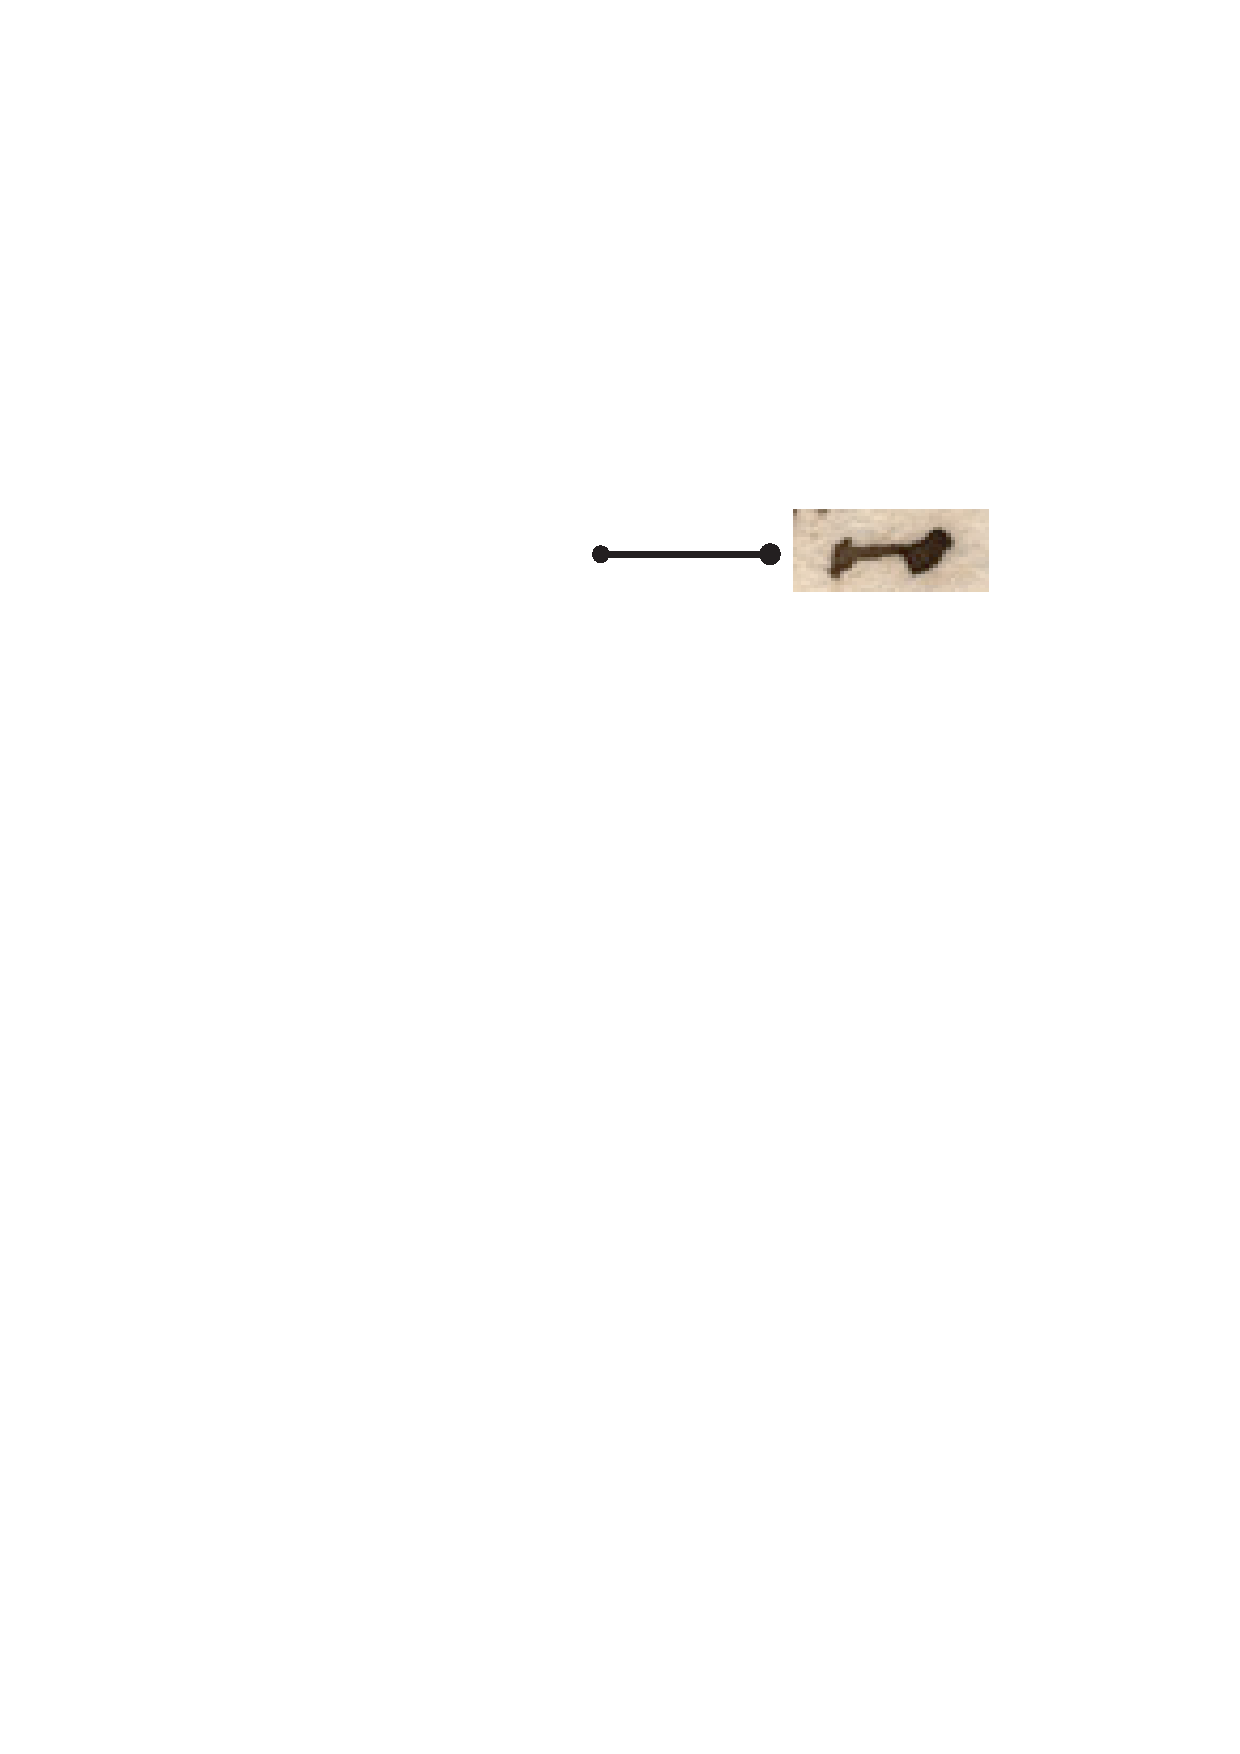
\includegraphics[width=0.15\textwidth]{images/lh0040104b_013r2.pdf}
quasdam etiam habentes aliquid in medio sic:
\rule[-2mm]{0mm}{9mm}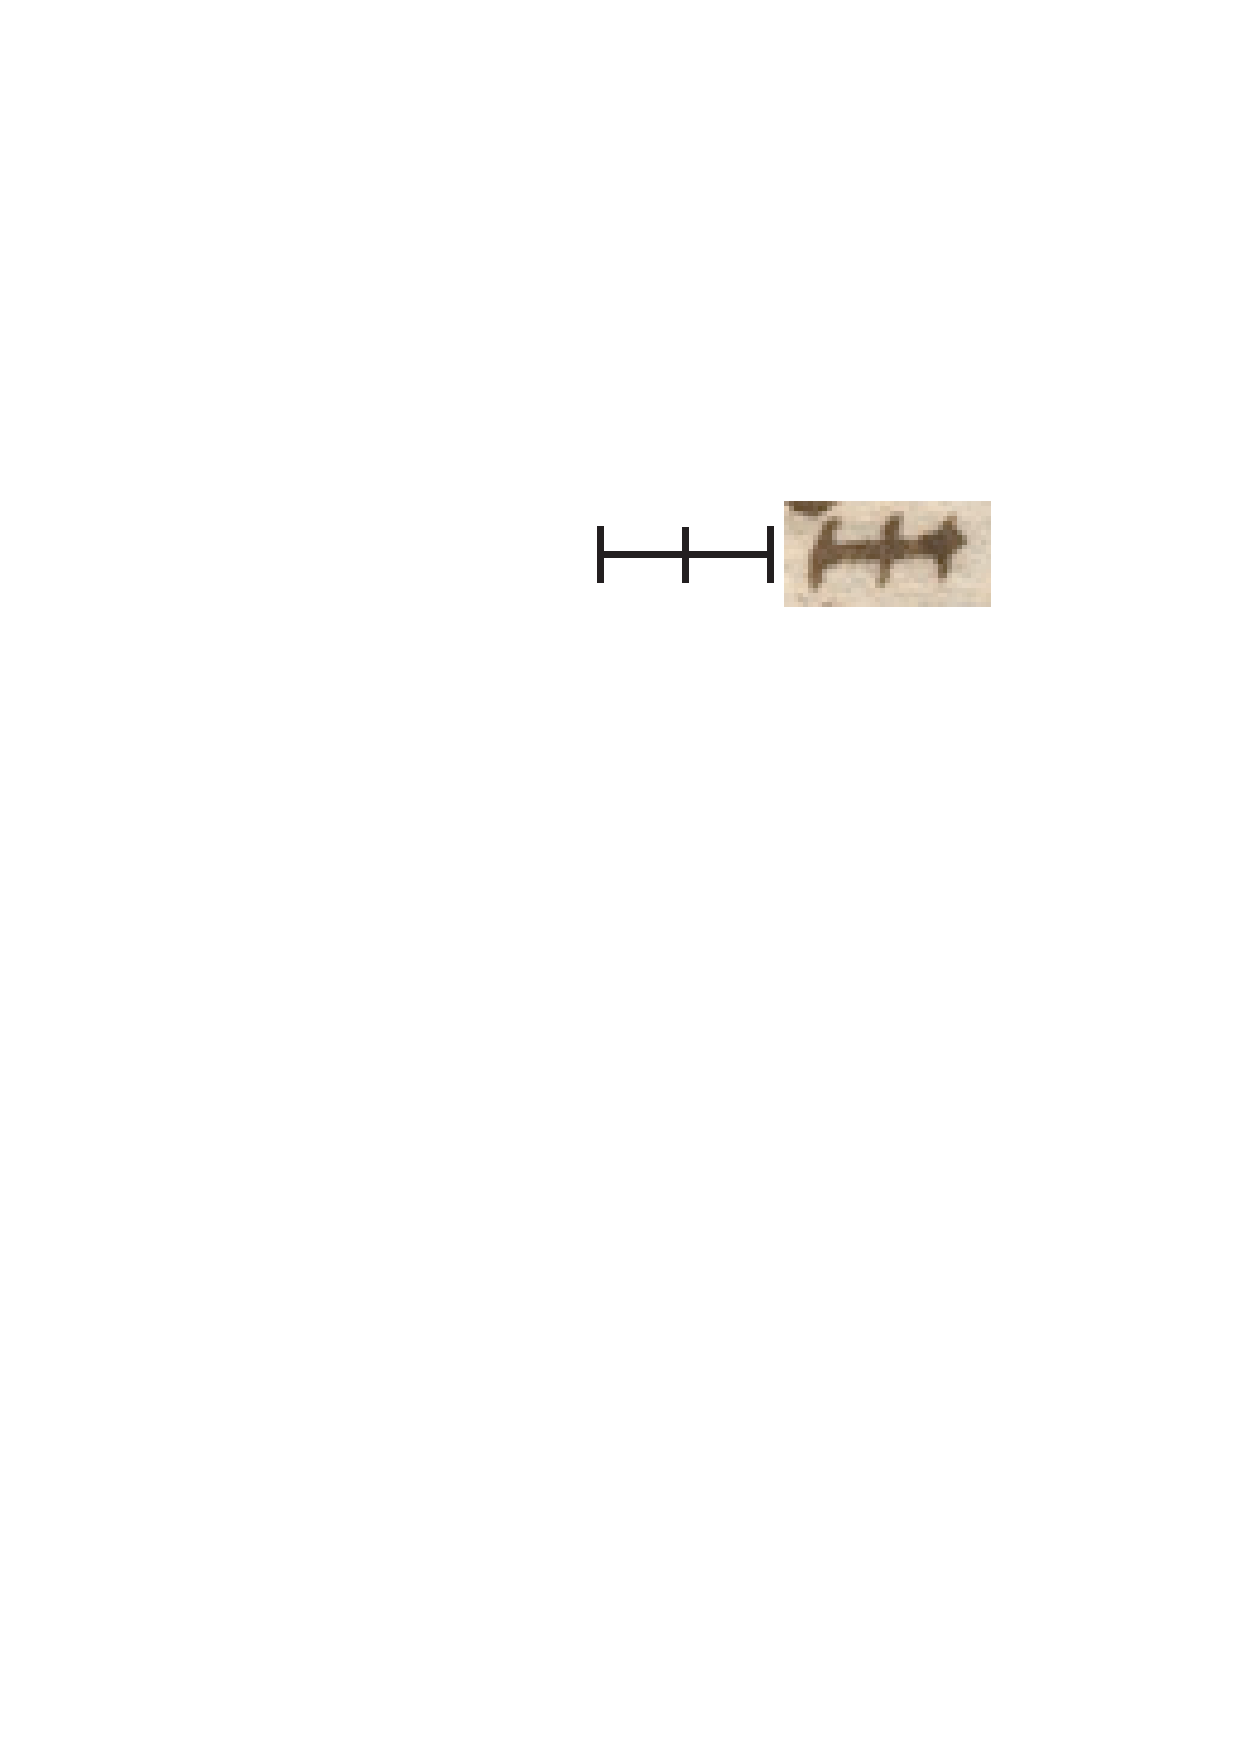
\includegraphics[width=0.15\textwidth]{images/lh0040104b_013r3.pdf},
non potui autem notare an quod in medio erat esset hexagonum; erant autem tam affabre factae, ut nihil magis. Paulatim vero ceciderant his breviores, in quarum una extremitate\label{extremitate} stella erat major quam in altera, et postea duplices cum 12 radiis interdum aeqalibus interdum non. Et unam vidi cujus uni radio columna cum alia minore stellula insidebat et
\edlabel{etquatuor}\edtext{}{{\xxref{etquatuor}{tranquillitate}}\lemma{et quatuor aut [...] tranquillitate}\Cfootnote{Textüberhang auf Bl.~13~v\textsuperscript{o}.}}%
quatuor aut 5 ex octo radiis factas, ita ut quatuor essent aliis breviores et appareret ex duabus factas esse sic: 
\rule[-2mm]{0mm}{10mm}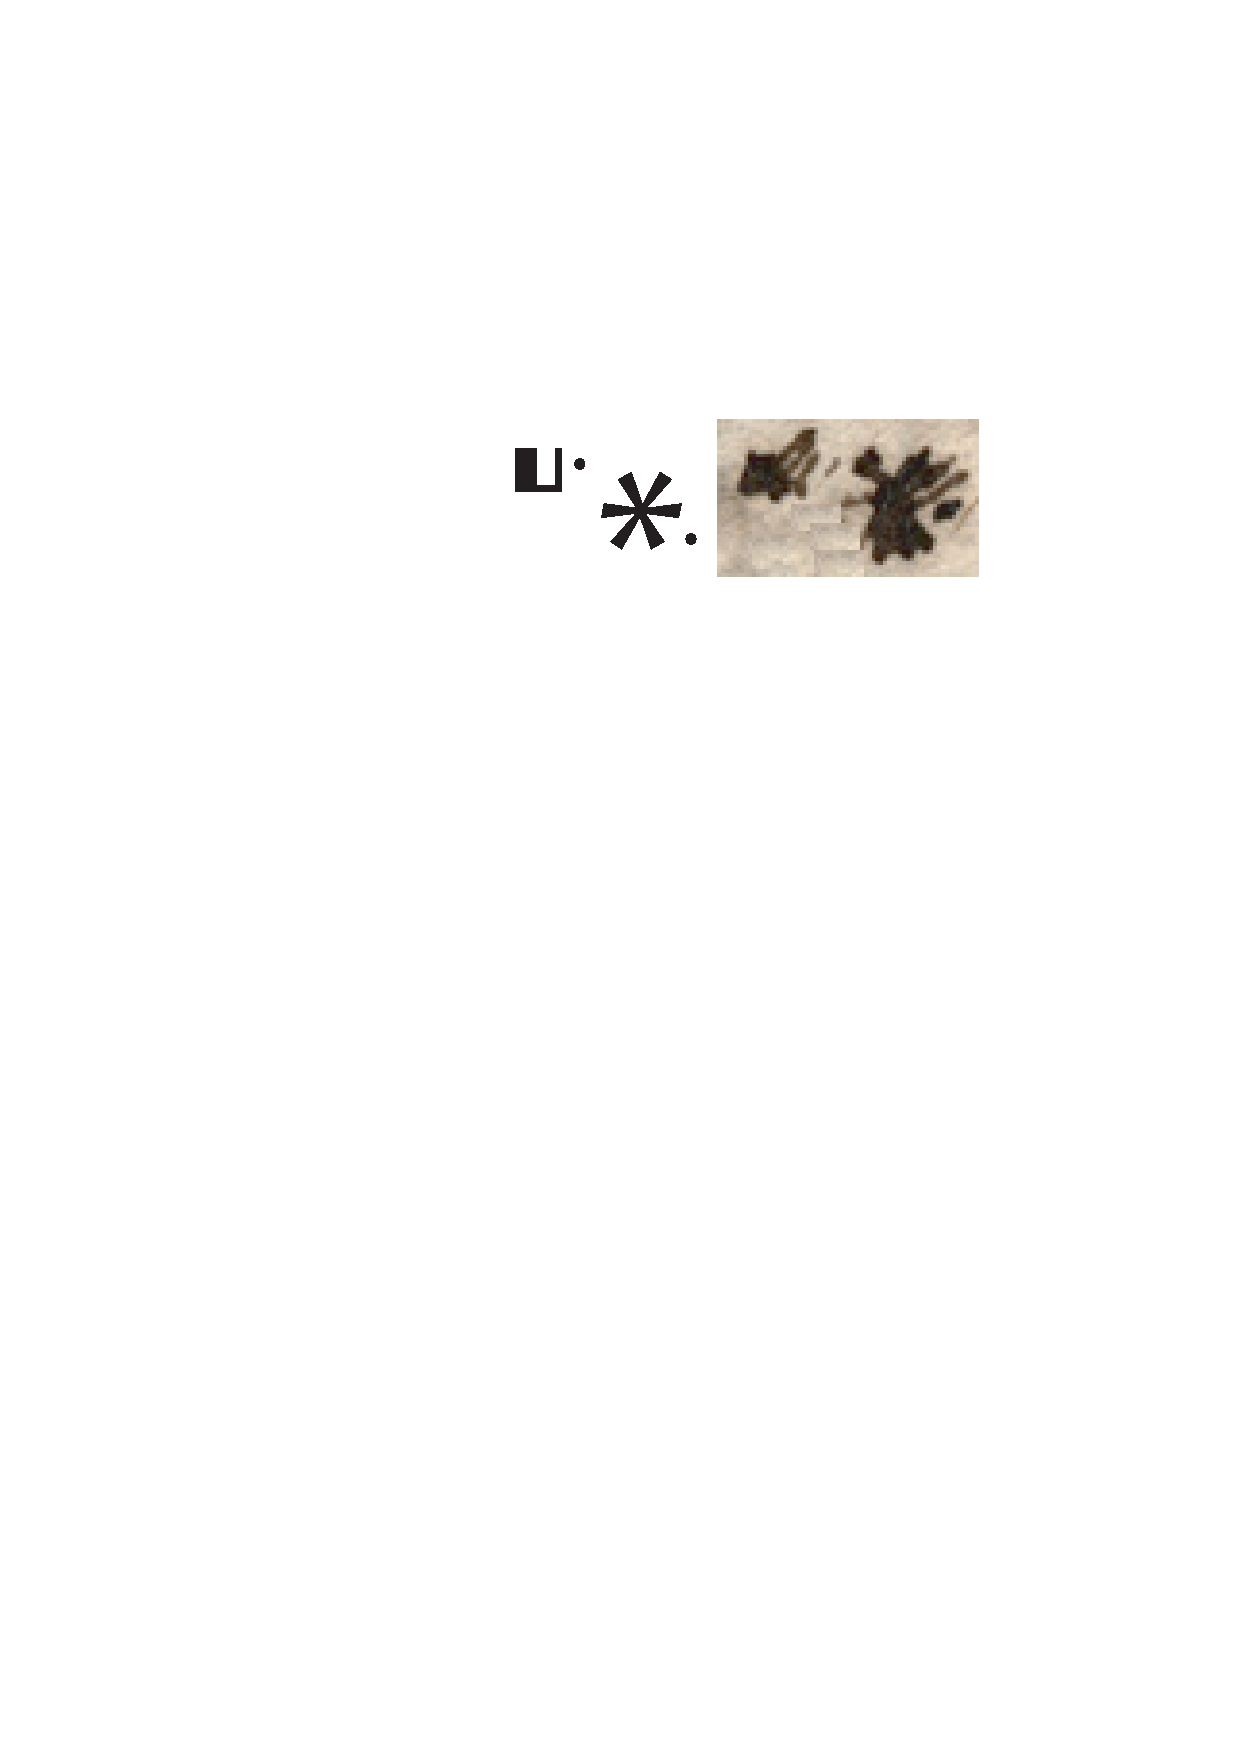
\includegraphics[width=0.15\textwidth]{images/lh0040104b_013v1.pdf}
Erant autem omnes tota die satis spissae, sed sub vesperem cum ningere desineret, erant multo tenuiores, et sequenti die mane, cum ventus mutaretur, et aura fieret serenior etiam stellulae 1\textsuperscript{o} tenuissimae, et in crassos floccos conglobatae paucae ceciderunt, deinde etiam aliae satis latae, sed non pellucidae, ac postea grandinis triangularis parum et aura serenior secuta est cum aeris
tranquillitate.\edlabel{tranquillitate} 
\pend%
\pstart%
Baculus aequaliter fortis utraque manu, arcus instar curvatus in medio inter manus intervallo frangetur, et quo manus ab invicem erunt remotiores eo facilius frangetur, quod utrinque sint quasi vectes hypomochlium habentes in loco ubi fit fractio.
\pend%
\pstart
Poma ex arboribus ita formantur, emergunt particulae ex trunco recto motu, quae deinde in orbem reflectuntur et fit alius motus circularis decussatim, cujus cum priori mistione\hfill particulae\hfill franguntur\hfill magis\hfill et\hfill magis,\hfill et\hfill ita\hfill fructus\hfill maturescit;\hfill paulatim\hfill vero
\pend
\newpage
\pstart%
\noindent iste motus circularis ipsam pomi caudam in orbem rodit, donec maturo fructu tota separetur et fructus cadat insitio vero vel etiam solius terrae cultura faciunt ut fructus
\edlabel{sint}\edtext{}{{\xxref{sint}{porosam}}\lemma{sint [...] porosam}\Cfootnote{Textüberhang auf Bl.~13~v\textsuperscript{o} und Bl.~14~r\textsuperscript{o}.}}%
sint mitiores, quia nempe particulae
\edtext{per [duarum] diversi}{\lemma{}\Bfootnote{per\ \textbar\ duorum \textit{\"{a}ndert Hrsg.}\ \textbar\ \textit{(1)}\ diverso \textit{(2)}\ diversi \textit{L}}}
generis arborum meatus evectae magis interpolantur. Item ex terra saepius versa subtiliores partes attrahuntur, quia si terra diu resederit in eodem loco paulatim ejus minutiae in easdem partes conspirabunt, adeo ut radices arborum similes sint iturae. Glebis autem saepe versis contra una arborem ingredietur uno modo
\edtext{alia alio}{\lemma{alia}\Bfootnote{\textit{(1)}\ alia \textit{(2)}\ alio \textit{L}}}
meliusque ibi miscebuntur. Dissimilia enim ut misceantur debent in plures partes frangi. Hinc fructus omnes sylvestres fiunt acerbi. Summatim vero sic plantae omnes prodeunt ex terra: copiosus vapor vi solis per unam terrae partem ascendit, atque circumjacente aere ejus motui resistente partim siccatur, partim ejus fibrae, quae in rectum surgebant, in transversum volvuntur, unde fit cortex, habens solum fibras transversas, cum e contra partes interiores habeant rectas si qui deinde meatus occurrant, in cortice, vapor inter hunc et lignum ascendens per istos meatus oblongos solum in transversum, eorum figuram sumit, et formatur in folia qui vero ex ipsa ligni medulla per lignum corticemque pervadit, quoniam inter fibras partim rotundas partim transversas egreditur, fit rotundus, atque ex eo concrescit primo oculus arboris, deinde flos, denique pomum,
ut \edtext{supra\edtext{, fit}{\lemma{supra,}\Bfootnote{\textit{(1)}\ vel \textit{(2)}\ fit \textit{L}}}}{\lemma{supra}\Cfootnote{Siehe oben, %LH IV 1,4B Bl. 13~\textsuperscript{o}r, Z. 70f, hier 
S. \pageref{extremitate}.}}
autem cavitas in medio omnium plantarum, vel aere vel medulla plena; quoniam partes vaporis non plane recta sursum, sed oblique hinc et inde, ut patet ex fibris lignorum quae ex iis sunt, solidiores versus corticem feruntur, manetque in medio quod levius est, ut sol inter planetas.
Plantae \edtext{[quae]}{\lemma{quae}\Bfootnote{\textit{erg. Hrsg.}}}
sub aquis nascuntur caeteris sunt magis fungosae et aereae quod vapor vi caloris per radices in plantam surgens est totus fere aereus, in plantis autem quae crescunt in aere facile illius vaporis
tenuioris partes expirant, manentque tantum sicciores ad constituendam plantam,
(quae etiam ideo solidior erit in monte quam in valle)
sub aquis vero istae partes aereae continuitate aquae et lentore quodam ejus naturae proprio retinentur, efficiuntque iccirco plantam magis
porosam.\edlabel{porosam}
[14~r\textsuperscript{o}]
\pend%
%%\newpage% PR: Rein provisorisch !!!
%\vspace*{1.5em}% PR: Rein provisorisch !!!
%% \begin{wrapfigure}{l}{0.6\textwidth}                    
%\pstart%
%\noindent%
%\centering%
%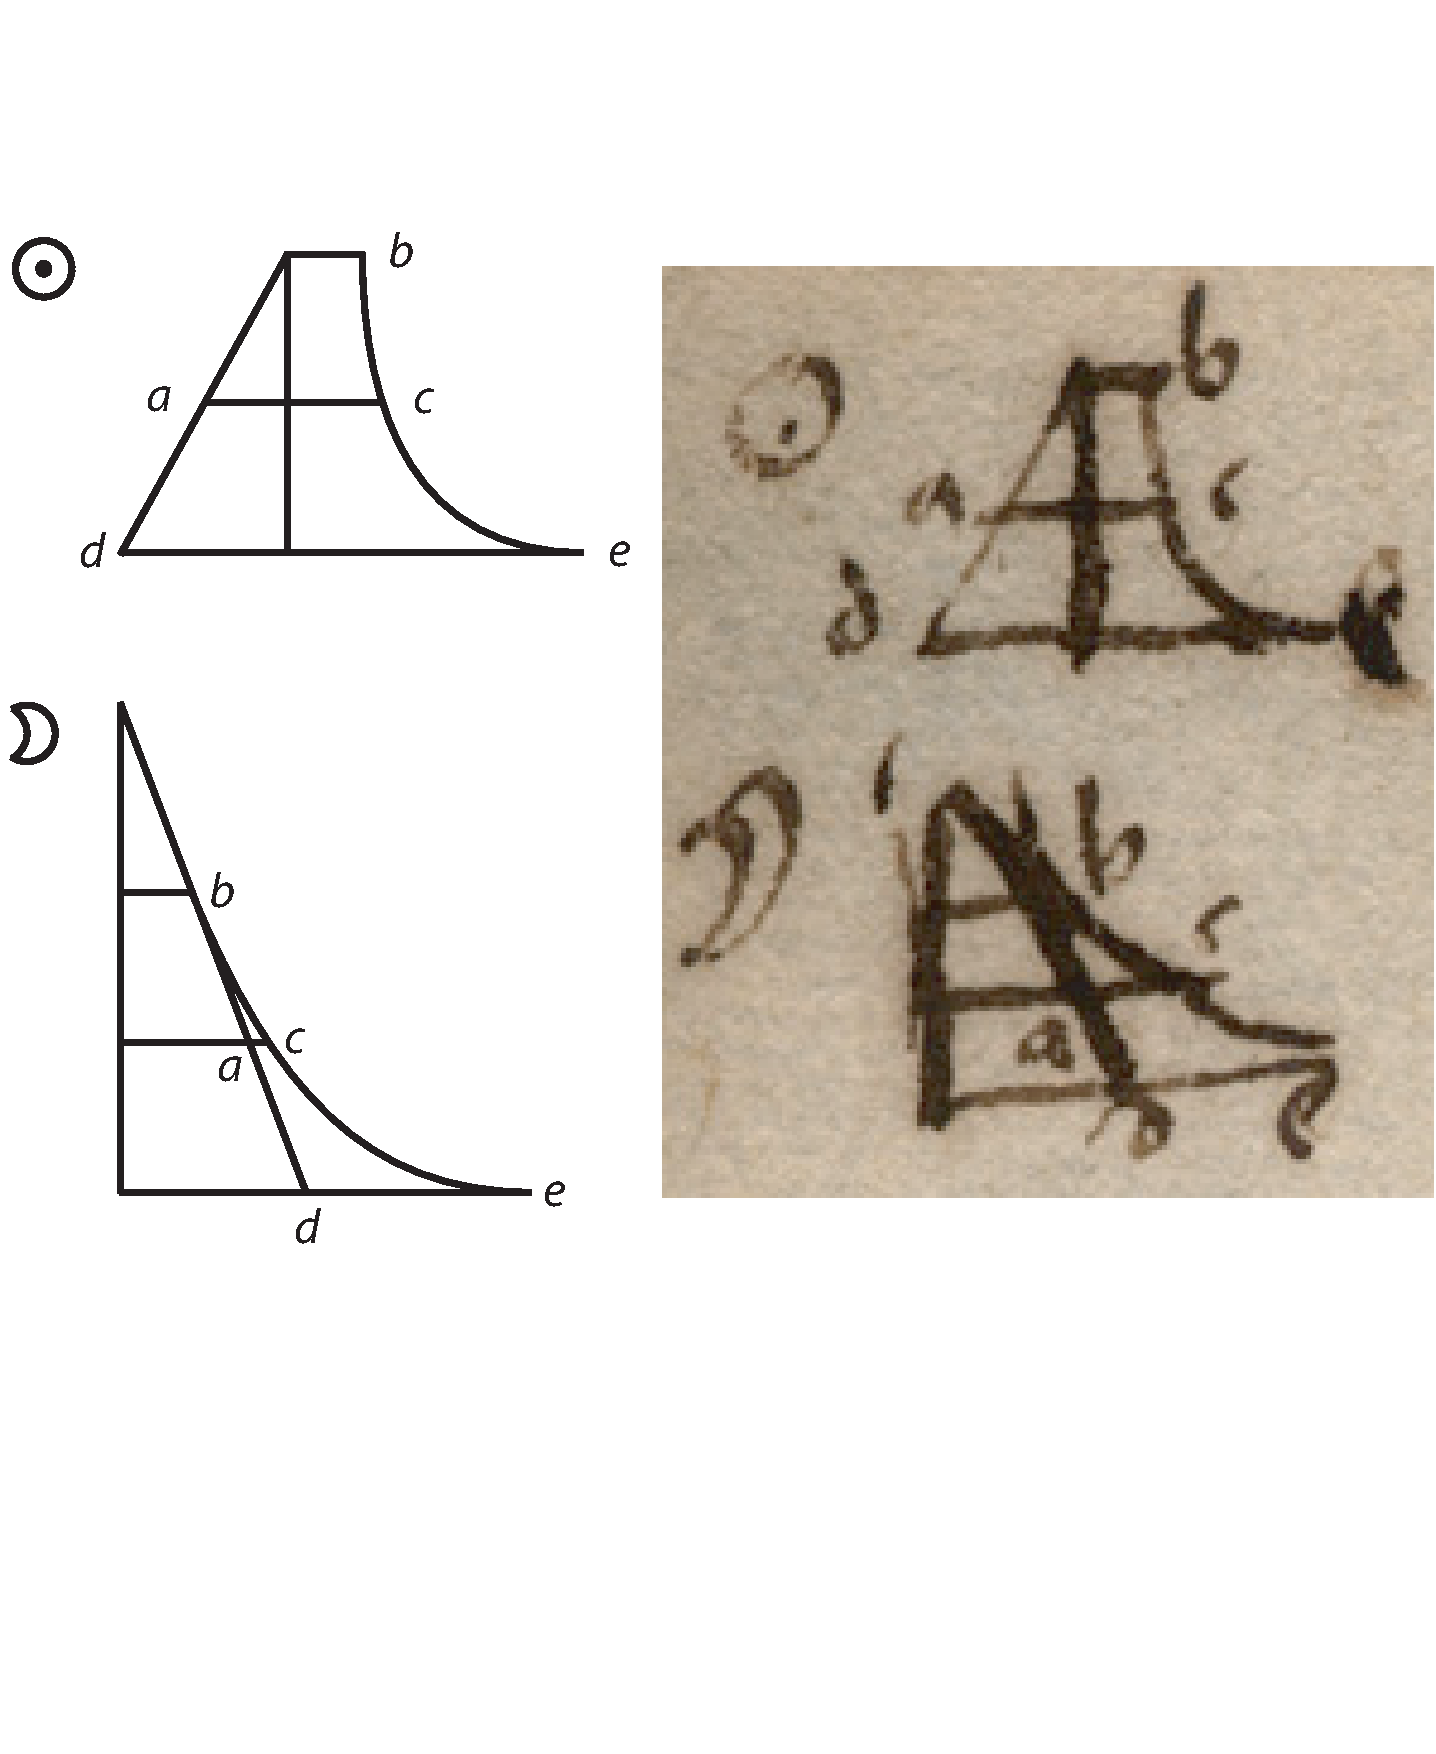
\includegraphics[width=0.75\textwidth]{images/lh0040104b_014v1u2.pdf}\\
%\rule[0mm]{0mm}{0mm}[\textit{Fig. 1}]
%%\caption{Bildbeschreibung}
%\pend%
%% \end{wrapfigure}
%\vspace*{1.5em}% PR: Rein provisorisch !!!
\pstart%
Si quod corpus ageretur sive impelleretur ad motum semper aequali vi nempe a mente sibi indita, (nulla enim alia vis talis esse potest) et moveretur in vacuo, semper a principio motus
\edtext{sui ad medium}{\lemma{}\Bfootnote{sui\ \textbar\ motus \textit{streicht Hrsg.}\ \textbar\ ad medium\ \textit{L}}}
spatii percurrendi triplo plus temporis poneret, quam a medio ad finem, et sic consequenter. Quia vero nullum tale vacuum dari potest, sed quodcunque\hfill spatium\hfill existat\hfill semper\hfill aliquo\hfill modo\hfill resistit;\hfill ista\hfill semper\hfill resistentia\hfill crescit
\pend
\newpage
\pstart%
\noindent%
\centering%
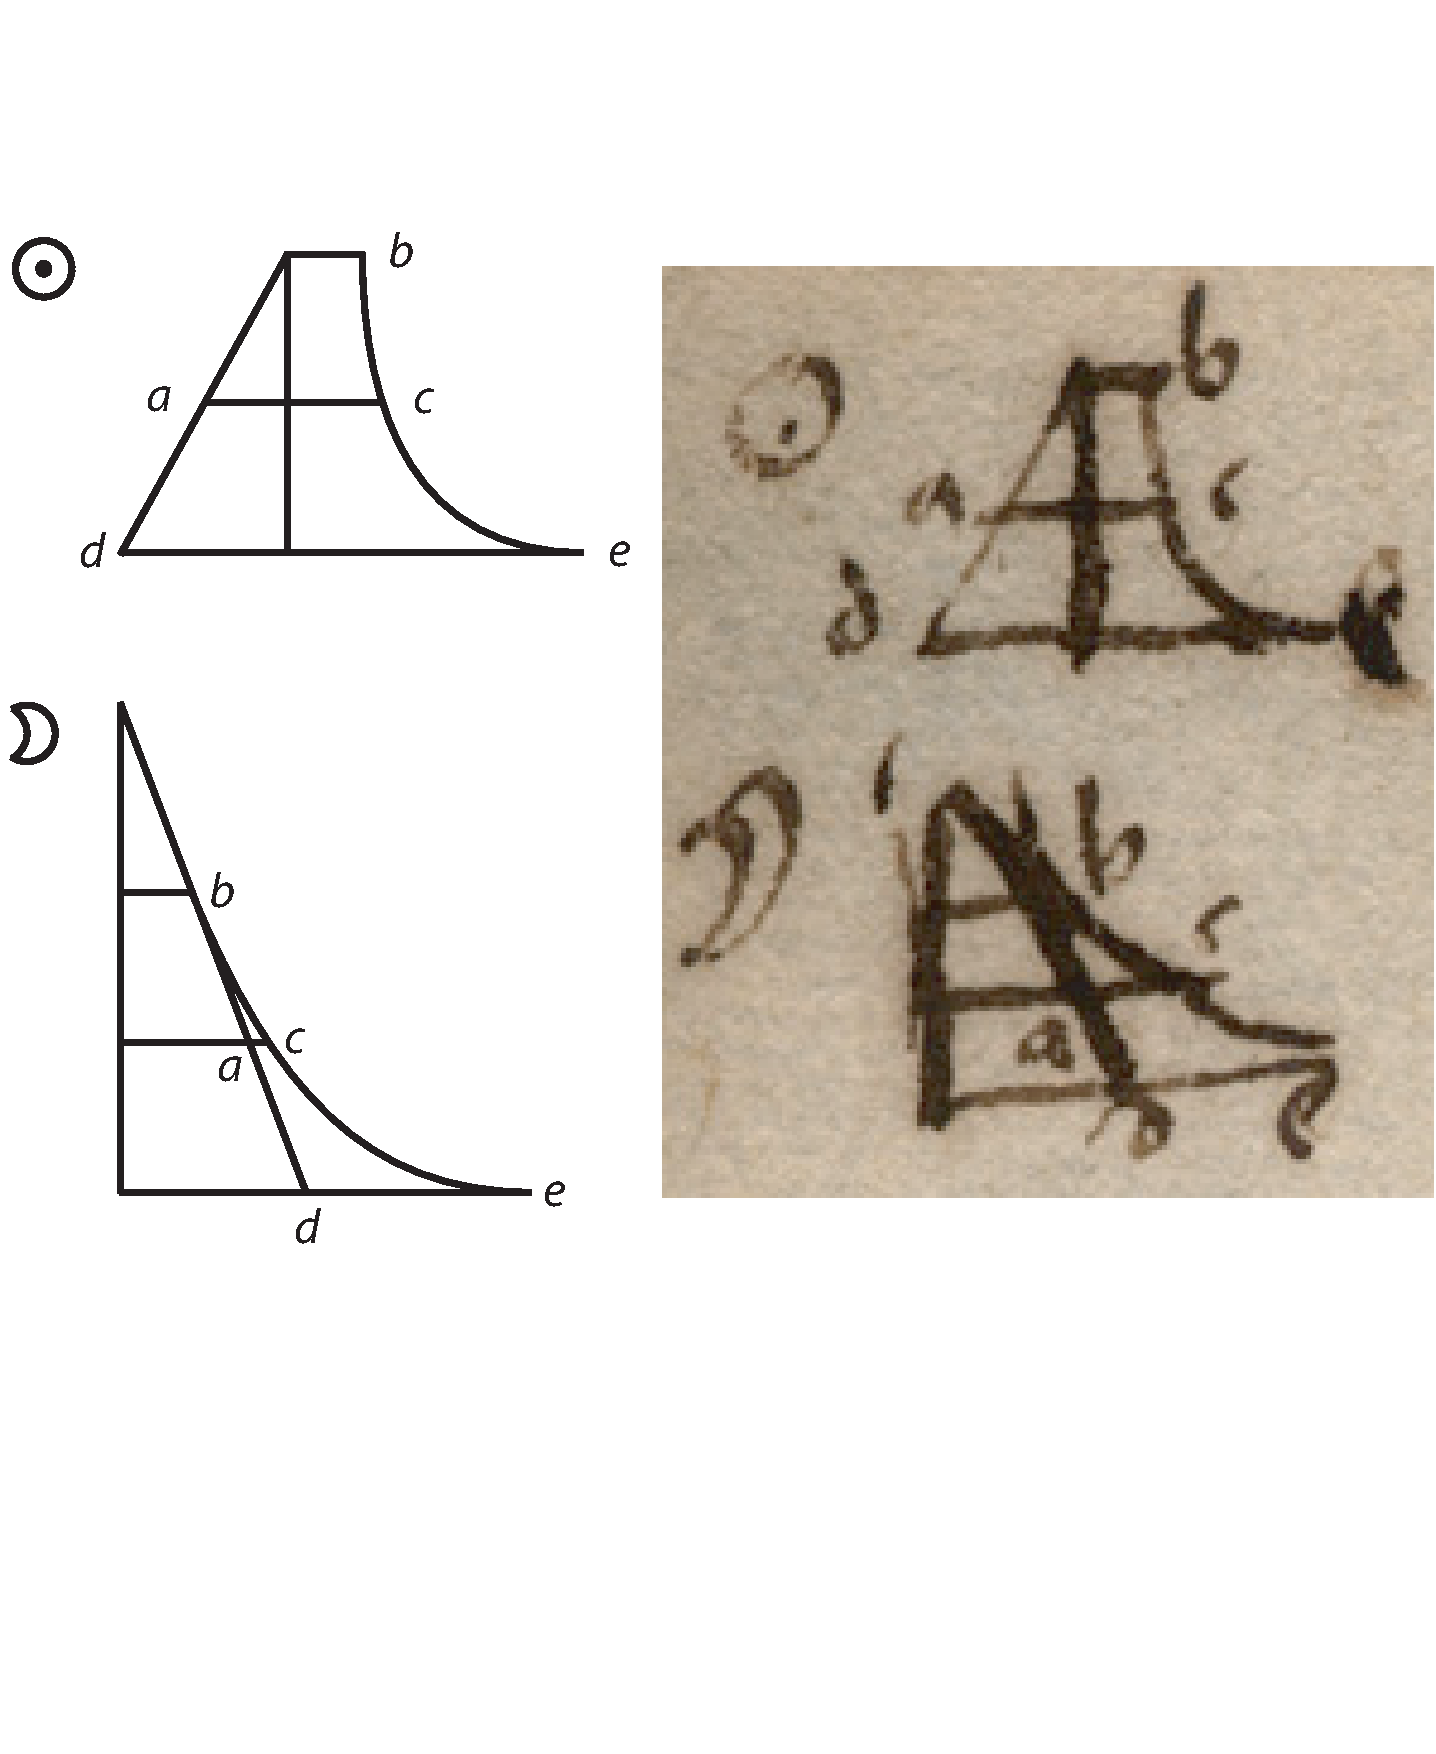
\includegraphics[width=0.75\textwidth]{images/lh0040104b_014v1u2.pdf}\\
\rule[0mm]{0mm}{0mm}[\textit{Fig. 1}]
\pend%
\vspace*{1.5em}
\pstart
\noindent
in proportione  \setline{1}Geometrica ad celeritatem motus, adeo ut eo tandem deveniatur ut non amplius sensibiliter augeatur celeritas, possitque determinari quaedam alia celeritas finita, cui nunquam erit aequalis. Quae a vi gravitatis impelluntur, cum ista gravitas non agat semper aequaliter tanquam anima, sed sit quoddam aliud corpus quod jam est in motu, nunquam potest rem gravem tam celeriter impellere quam
\edtext{ipsum movetur,}{\lemma{ipsum}\Bfootnote{\textit{(1)}\ moveatur \textit{(2)}\ movetur, \textit{L}}} sed etiam in vacuo minueretur semper impulsus in
\edtext{proportione \edlabel{Geometrica}Geometrica}{\lemma{}\Bfootnote{proportione\ \textbar\ Geometrica ad celeritatem motus adeo ut eo tandem perveniatur, ut non amplius sensibiliter augeatur celeritas possitque determinari quaedam alia celeritas finita cui nunquam erit aequalis. Quae a vi gravitatis impelluntur, cum ipsa gravitas non agat semper aequaliter tanquam anima, sed sit quoddam aliud corpus quod jam est in motu, nunquam potest rem gravem tam celeriter impellere quam ipsum movetur sed etiam in vacuo minueretur semper impulsus in proportione \textit{gestr.}\ \textbar\ Geometrica \textit{ L}}}\edtext{}{{\xxref{Geometrica}{aced}}\lemma{Geometrica quae [...] spatium $aced$}\Cfootnote{Textüberhang auf Bl.~14~v\textsuperscript{o}.}}
quae vero mi\-nu\-untur a duabus causis vel pluribus in proportione Geometrica minuuntur ab illis omnibus tanquam ab una causa quae illa minueret in proportione Geometrica, semperque redit eadem supputatio; item etiam, si quae alia causa retineat vi arithmetica consurget semper diminutio in proportione Geometrica, si vero aliqua alia vis impellat%
\edtext{}{\lemma{}\Afootnote{\textit{Am Rand:} (+ Ergo NB vis animae in vacuo arithmetica +)}}
semper in proportione Geometrica simul agens cum ea quae Geometrice minuitur, eo tandem pervenietur, ut Geometrica cesset solaque arithmetica remaneat augeatque motum ut dictum est facturam animam in vacuo.
Quid agitur si crescat impulsus Geometrice, et minuatur vel crescat etiam arithmetice, crescet celeritas in infinitum proportione
\edtext{composita, quae}{\lemma{}\Bfootnote{composita\ \textbar\ composita \textit{streicht Hrsg.}\ \textbar\ , quae \textit{L}}}
pot\-est explicari per spatia ope trianguli et
\edtext{[areae]}{\lemma{areeae}\Bfootnote{\textit{L \"{a}ndert Hrsg.}}}
linea proportionalium comprehensae hoc modo \astrosun\ addendo vel hoc $\rightmoon$ detrahendo, ita ut celeritas primi temporis sit ad celeritatem secundi, ut spatium $abc$ ad spatium $aced.$\edlabel{aced}
\pend%
\pstart%
Notavi pyxidem optime clausam in qua fuerat aqua odorata per totum hyemem, cum vere illam aperui, aquam cum quodam impetu exiliisse, nempe hyeme partes densae frigore fuerant in eam introductae, quas veris calor non tam facile expellebat, ideoque aqua ista erat intus quasi compressa, idem in omnibus fere fieri puto, ut veris calor, cum non facile rarefiat ea quae hyeme densata sunt, id efficere cum quodam impetu, cum eousque crevit, ut praevaleat, et hunc impetum ad eorum quae
\edtext{vere}{\lemma{}\Afootnote{\textit{\"{U}ber} vere: verno tempore}}
generantur ortum conferre
\edtext{existimo. Dum}{\lemma{existimo.}\Bfootnote{\textit{(1)}\ Dum vina nova aut cerevisiae bulliunt hoc fit \textit{(2)}\ Dum \textit{L}}}
vina nova aut cerevisiae bulliunt, hoc fit ex contrarietate motuum qui
\edtext{sunt inter}{\lemma{sunt}\Bfootnote{\textit{(1)}\ in ipsis \textit{(2)}\ inter \textit{ L}}}
eorum partes%
%%%%
\edtext{}{\lemma{}\Afootnote{\textit{Am Rand:}
[Contraria]\textsuperscript{[a]}
simul complicata se invicem etiam\textsuperscript{[b]}
comburere dicit Hippocrates\textsuperscript{[c]}
(+~margini adscriptum~+).%
\vspace{1mm}% PR: Rein provisorisch !!!
\newline%
\footnotesize%
%
\textsuperscript{[a]}
Coria\ \textit{L \"{a}ndert Hrsg.}
\quad
%
\textsuperscript{[b]}
etiam\ \textbar\ etiam \textit{streicht Hrsg.}\ \textbar\ comburere\ \textit{ L}
\quad
%
\textsuperscript{[c]}
Hippocrates: \cite{01143}\textit{De victu} % (\pgrk{Per‘i dia’ijhs}) 
I.5 (Littré VI, S. 478.4).\vspace{-6mm}%
}}
%%%%
quae proinde locum ampliorem requirunt, et fluidas particulares inter se, velut in angulis contingentiae admittunt; unde oritur calor, ita quoque fit concoctio alimenti in ventriculo animalium. Ut calx et aqua neutrum est calidum separatim, ita etiam vinum ex uvis statim eductum non bulliret, sed tantum quod per aliquod tempus cum racemis maceratur, ex quorum contraria natura hunc calorem accipit, cujus agitatione postea perfectius miscetur, atque adeo minus facile corrumpi potest; mutuatur enim quasi quosdam nervos a
\edtext{[racemorum]}{\lemma{ramorum}\Bfootnote{\textit{L \"{a}ndert Hrsg.}}}
duritie, quibus materia fluida, firmatur et
\edtext{[contra]}{\lemma{circa}\Bfootnote{\textit{L \"{a}ndert Hrsg.}}}
aeris circumjacentis motus ad corruptionem tendentes defenditur.
\pend%
\pstart%
Dicimus aerem multa
\edtext{mixta corrumpere potius, quam}{\lemma{mixta}\Bfootnote{\textit{(1)}\ generare potius quam \textit{(2)}\ corrumpere potius, quam \textit{L}}}
generare, contra solem dicimus ea generare potius quam corrumpere, quod vel ideo fit, quia motus aeris est imbecillus, et in diversas partes sive inordinatus, et proinde quae ab eo sunt alterata non habent facultatem conservandi sui in eodem statu, ideoque non dicimus
\edtext{ea habere}{\lemma{ea}\Bfootnote{\textit{(1)}\ esse \textit{(2)}\ habere \textit{L}}}
formas perfectas, sed esse tantum res corruptas; contra vero solis motus est uniformis sive ordinatus et fortior, et proinde quae ab illo formam acceperunt, plerumque illam habent magis durabilem, quanquam hoc variet frequenter propter dispositiones subjecti.
\pend%
\pstart%
Senes habent \textso{capillos} albos, et animalia in frigidis regionibus nata albos pilos, contra Aethiopes nigerrimos, idem etiam de cute, quod fit quoniam calore intus et extra majore existente, excrementa ista ex corpore exeuntia saepius interrumpunt fluxum suum quae interruptio nigrum calorem efficit, facit etiam ut Mauri intortos et mollissimos habeant capillos, contra in aliis regionibus minor calor crassiores particulas emittit, quae singulae cum sint pellucidae satis duntaxat interrumpuntur ad efficiendum album colorem, non nigrum, et crassos capillos non tenues ut Maurorum.
\pend%
\pstart%
Pilos crispos fieri certum est, quod cuticula proportione densior est quam cutis cumque radices agant in cute per cuticulam transeuntes, oblique inflectuntur; patet Aethiopes istam cuticulum habere densiorem, quod calido aere siccatur; aetate autem cuticulae meatus augentur, et saepe qui in juventute crispi erant non sunt amplius in senectute; contra fieri potest ut morbo lapsis crinibus ista cuticula densetur, crispique renascantur, cum prius fuissent plane recti quod in quodam observavi.
\pend%
\count\Bfootins=1500
\pstart%
\edtext{Pili in ciliis nascuntur in utero, quod ibi materiam habent aptam, nempe cartilaginem nondum duratam, non vero crescunt postea, quod durata
\edtext{ista cartilago}{\lemma{ista}\Bfootnote{\textit{(1)}\ cartilagine \textit{(2)}\ cartilago \textit{L}}}
non amplius apta est emittendis pilis, nisi forte senectute laxata. \\ Pilorum materia est quod excernitur lentum vel siccum ex cerebro vel glandulis, et similibus subjectis, cujus naturae cartilagines initio esse cilia testantur. (+~per dicta~+)}{\lemma{Pili in [...] dicta~+\phantom(\hspace{-1.2mm})}\Cfootnote{Textüberhang auf Bl.~14~v\textsuperscript{o}.}}
\pend%
\pstart%
Lacrymae sunt sudor oculorum quod patet ex eo quod omnis res oculos calefaciens elicit lacrymas.
\pend%
\pstart%
Sudor non differt ab ea materia quae exhalat e corpore per insensibiles transpirationes, nisi copia, cruditate, et salsedine, quia cum magis laxentur meatus cutis, fit aqua quod alioqui esset aer, sed cera in oculis est lentor sudoris, ut pili et furfures la crasse, sudant quippe multum glandulae et cerebrum, quodque exudat lentius et crassius est. Urina est eadem pars sanguinis per renem interpolata, qualis est sudor per cutem, nisi quod paulo crassior sit. Ex lacte tria excernuntur, serum, pingue seu butyrum, et siccum cutem
\edtext{caill\'{e}.}{\lemma{caill\'{e}}\Bfootnote{\textit{erg. L}}}
\pend%
\pstart%
Saccarum est sal glutinosum, atque si quod glutinosum est ex saccaro tolleretur, salsum remaneret; sanguis eodem modo dulcis est, et quicquid est in eo glutinosum, abit in carnes, ideo residuus sudor est salsus. Nimirum sudor ideo salsus est, quia cum sit ea sanguinis pars quae non facessit in carnes, nihil autem salis agglutinetur carnibus propter suam siccitatem, qua potius
\edtext{[eas]}{\lemma{eos}\Bfootnote{\textit{L \"{a}ndert Hrsg.}}}
corroderet, ideo totus sal in sanguine existens, redundat in sudorem et in urinas.
\pend%
\pstart%
\textso{Problemata }promiscua: quare glacies non liquescit gradatim mollescendo ut cera (+~nihil ascriptum ultra erat, nec alia problemata sequuntur~+).
\pend%
\count\Bfootins=1500
\count\Cfootins=1500
\count\Afootins=1500
% ENDE